% ============================================================
% LAPORAN PRAKTIKUM ALGORITMA DAN PEMROGRAMAN
% Modul 5: Fungsi, Parameter, dan Nilai Kembalian
% Compile dengan pdfLaTeX
% ============================================================

\documentclass[12pt,a4paper]{article}

% ---------- Font sederhana ----------
\usepackage[T1]{fontenc}
\usepackage[utf8]{inputenc}
\usepackage{mathptmx}

% ---------- Tata letak ----------
\usepackage[a4paper,left=3cm,right=2cm,top=2cm,bottom=2cm]{geometry}
\usepackage{setspace}
\setstretch{1.15}
\usepackage{ragged2e}
\justifying
\setlength{\parindent}{1.25cm}
\setlength{\parskip}{0pt}

% ---------- Paket umum ----------
\usepackage{graphicx}
\usepackage{float}
\usepackage{enumitem}
\usepackage{titlesec}
\usepackage{array}
\usepackage{booktabs}
\usepackage{longtable}
\usepackage{caption}
\usepackage{hyperref}
\usepackage{amsmath}
\hypersetup{hidelinks}

% ---------- Format heading ----------
\titleformat{\section}
  {\bfseries\fontsize{12pt}{14pt}\selectfont}
  {}{0pt}{}
\titlespacing*{\section}{0pt}{12pt}{6pt}

\titleformat{\subsection}
  {\bfseries\fontsize{12pt}{14pt}\selectfont}
  {}{0pt}{}
\titlespacing*{\subsection}{0pt}{10pt}{4pt}

\titleformat{\subsubsection}
  {\bfseries\fontsize{12pt}{14pt}\selectfont}
  {}{0pt}{}
\titlespacing*{\subsubsection}{0pt}{8pt}{3pt}

\setlist[enumerate]{leftmargin=1.1cm,itemsep=0pt,topsep=2pt}
\setlist[itemize]{leftmargin=1.1cm,itemsep=0pt,topsep=2pt}

% ---------- Helper template ----------
\newcommand{\placeholder}[1]{\textit{[#1]}}
\newcommand{\imageplaceholder}[1]{%
  \begin{center}
  \fbox{\parbox[c][5.5cm][c]{0.88\textwidth}{\centering\textit{[#1]}}}
  \end{center}
}

\begin{document}

% ============================================================
% COVER
% ============================================================
\begin{titlepage}
\thispagestyle{empty}
\begin{center}

{\bfseries\fontsize{16pt}{19pt}\selectfont LAPORAN PRAKTIKUM\par}
\vspace{0.25cm}
{\bfseries\fontsize{16pt}{19pt}\selectfont ALGORITMA DAN PEMROGRAMAN\par}
\vspace{0.45cm}
{\bfseries\fontsize{14pt}{17pt}\selectfont MODUL 5\par}
\vspace{0.15cm}
{\bfseries\fontsize{14pt}{17pt}\selectfont FUNGSI, PARAMETER, DAN NILAI KEMBALIAN\par}

\vspace{1.2cm}

\IfFileExists{logo_telkom_university.png}{%
  
\includegraphics[width=0.34\textwidth]{logo_telkom_university.png}%
}{%
  \IfFileExists{../logo_telkom_university.png}{%
    \includegraphics[width=0.34\textwidth]{../logo_telkom_university.png}%
  }{%
    \IfFileExists{../../logo_telkom_university.png}{%
      
\includegraphics[width=0.34\textwidth]{../../logo_telkom_university.png}%
    }{%
      \fbox{\parbox[c][3.5cm][c]{0.34\textwidth}{\centering\textit{[Logo Telkom University]}}}%
    }%
  }%
}

\vspace{1.2cm}

\renewcommand{\arraystretch}{1.35}
\begin{tabular}{>{\bfseries}p{2.3cm} p{0.35cm} p{8.4cm}}
NAMA  & : & DENDRA DE TAMA \\
NIM   & : & 108052600034 \\
KELAS & : & SS1SI-50-REG-01 \\
PRODI & : & S1 SISTEM INFORMASI \\
\end{tabular}

\vfill

{\bfseries TELKOM UNIVERSITY SURABAYA\par}
{\bfseries FAKULTAS REKAYASA INDUSTRI\par}
{\bfseries PROGRAM STUDI S1 SISTEM INFORMASI\par}
\vspace{0.2cm}
{\bfseries TAHUN AKADEMIK 2025/2026\par}

\end{center}
\end{titlepage}

% ============================================================
% PENDAHULUAN
% ============================================================
\section{PENDAHULUAN}
Seiring dengan bertambahnya kompleksitas persoalan komputasi, penyusunan seluruh instruksi ke dalam satu alur sekuensial tunggal (\textit{monolithic code}) menjadi tidak efisien, sulit dipelihara, dan rentan menimbulkan redundansi kode. Untuk mengatasi tantangan tersebut, paradigma rekayasa perangkat lunak mengadopsi konsep pemrograman modular (\textit{modular programming}). Dalam bahasa Python, modularisasi diimplementasikan secara fundamental melalui perancangan fungsi (\textit{functions}).

Fungsi adalah blok kode terorganisir dan dapat digunakan kembali (\textit{reusable}) yang dirancang untuk menjalankan suatu tugas spesifik. Penerapan fungsi berpegang pada prinsip baku \textit{Don't Repeat Yourself} (DRY), di mana logika yang sama tidak ditulis berulang kali, melainkan diisolasi dalam satu definisi bernama. Dalam Python 3, fungsi dideklarasikan menggunakan kata kunci \texttt{def}, diikuti oleh nama fungsi, tanda kurung yang memuat daftar parameter formal, dan diakhiri dengan titik dua (\texttt{:}) serta blok tubuh fungsi yang diindentasikan.

Berdasarkan sifat keluarannya, fungsi terbagi menjadi dua kategori utama:
\begin{enumerate}
    \item \textbf{Prosedur (\textit{Void Function})}: Fungsi yang bertugas menjalankan serangkaian tindakan (seperti memformat dan mencetak teks ke layar) tanpa menghasilkan nilai data kembali untuk diolah lebih lanjut. Dalam arsitektur internal Python, fungsi jenis ini secara implisit mengembalikan objek khusus bernilai \texttt{None}.
    \item \textbf{Fungsi dengan Nilai Kembalian (\textit{Value-Returning Function})}: Fungsi yang mentransmisikan hasil komputasinya kembali ke pemanggil fungsi melalui kata kunci \texttt{return}. Penggunaan \texttt{return} secara seketika menghentikan eksekusi tubuh fungsi dan menyerahkan nilai objek ke pemanggil, sehingga hasilnya dapat ditampung ke dalam variabel, dievaluasi dalam ekspresi aritmatika, atau diumpankan langsung ke fungsi lain (*function composition*).
\end{enumerate}

Konsep penting lainnya mencakup lingkup hidup variabel (\textit{variable scope}). Variabel yang didefinisikan di dalam tubuh fungsi bersifat lokal (\textit{local scope}) dan disimpan di dalam bingkai tumpukan memori (\textit{stack frame}) fungsi tersebut. Variabel lokal hanya dapat diakses selama fungsi berlangsung dan akan dimusnahkan seketika setelah fungsi selesai dieksekusi, sehingga terisolasi sempurna dari variabel bernama sama di lingkup global (\textit{global scope}).

Selain fungsi komputasi standar, modul ini mendalami penerapan fungsi predikat bertipe boolean (*boolean-returning predicate*), integrasi pustaka bawaan Python (\textit{standard library modules}) seperti \texttt{math} untuk perhitungan analitik serta \texttt{random} untuk pembangkitan bilangan acak, dan paradigma komputasi rekursif (\textit{recursion}). Rekursi adalah teknik di mana suatu fungsi memanggil dirinya sendiri untuk menyelesaikan sub-masalah yang lebih kecil, yang mutlak mensyaratkan adanya kondisi berhenti (*base case*) yang ketat agar tidak menimbulkan luapan tumpukan memori (*stack overflow* atau galat \texttt{RecursionError}).

Praktikum Modul 5 ini mencakup lima latihan terstruktur dan satu studi kasus integratif, meliputi prosedur pencetakan kartu nama (\texttt{latihan1.py}), fungsi kalkulasi konversi suhu dan geometri (\texttt{latihan2.py}), fungsi predikat kelulusan dan pemutusan dini grade huruf (\texttt{latihan3.py}), integrasi fungsi jarak Euclidean dan simulasi dadu acak (\texttt{latihan4.py}), fungsi rekursif faktorial dan hitung mundur (\texttt{latihan5.py}), serta perancangan aplikasi modular kalkulator nilai akhir mahasiswa (\texttt{studi\_kasus.py}).

\subsection{Tujuan Praktikum}
\begin{enumerate}
    \item Memahami konsep modularisasi perangkat lunak dan sintaksis pendefinisian fungsi (\texttt{def}) serta mekanisme pelewatan parameter pada Python 3.
    \item Mengidentifikasi perbedaan arsitektural dan fungsional antara prosedur pencetakan (\textit{void function}) dan fungsi bernilai kembali (\texttt{return}).
    \item Mengimplementasikan fungsi predikat bertipe boolean dan teknik pemutusan eksekusi instan (*early return*) di dalam struktur percabangan.
    \item Memanfaatkan modul pustaka standar Python (\texttt{math} dan \texttt{random}) di dalam pembuatan fungsi komputasi kustom.
    \item Memahami mekanisme kerja fungsi rekursif, identifikasi kasus basis (*base case*), dan analisis pencegahan galat luapan rekursi (*stack overflow*).
    \item Merancang aplikasi komputasi modular berskala menengah melalui komposisi fungsi validasi masukan, perhitungan nilai terbobot, dan pelindung pembagian nol.
\end{enumerate}

% ============================================================
% LANGKAH PERCOBAAN
% ============================================================
\section{LANGKAH--LANGKAH PERCOBAAN}

\subsection{Percobaan 1: Prosedur dan Komposisi Fungsi (latihan1.py)}
\begin{enumerate}
    \item Pemahaman Persoalan: Program mendemonstrasikan perancangan prosedur tanpa nilai kembalian untuk mencetak elemen dekoratif dan kartu identitas mahasiswa. Prosedur \texttt{cetak\_garis} menerima parameter panjang garis dan mencetak karakter sama dengan ($=$) sebanyak panjang tersebut. Prosedur \texttt{kartu\_nama} menerima parameter nama dan prodi, lalu memanggil prosedur \texttt{cetak\_garis} untuk membingkai data identitas secara terstruktur.
    \item Data Masukan/Keluaran:
    \begin{itemize}
        \item Masukan: Tidak ada masukan dinamis dari konsol (parameter diumpankan secara langsung saat pemanggilan fungsi: nama \texttt{"Rani"} dan \texttt{"Dimas"} dengan program studi \texttt{"Sistem Informasi"}).
        \item Keluaran: Dua blok tampilan kartu nama rapi yang dibingkai oleh garis pembatas sepanjang 30 karakter.
    \end{itemize}
    \item Penyusunan Algoritma:
    \begin{enumerate}[label=\alph*.]
        \item Mulai program.
        \item Definisikan fungsi prosedur \texttt{cetak\_garis(panjang)}:
        \begin{itemize}
            \item Cetak string \texttt{"="} yang dikalikan dengan nilai parameter \texttt{panjang}.
        \end{itemize}
        \item Definisikan fungsi prosedur \texttt{kartu\_nama(nama, prodi)}:
        \begin{itemize}
            \item Panggil \texttt{cetak\_garis(30)}.
            \item Cetak label dan nilai parameter: \texttt{"Nama  :", nama}.
            \item Cetak label dan nilai parameter: \texttt{"Prodi :", prodi}.
            \item Panggil kembali \texttt{cetak\_garis(30)}.
        \end{itemize}
        \item Panggil prosedur \texttt{kartu\_nama("Rani", "Sistem Informasi")}.
        \item Panggil prosedur \texttt{kartu\_nama("Dimas", "Sistem Informasi")}.
        \item Selesai.
    \end{enumerate}
\end{enumerate}

\subsection{Percobaan 2: Fungsi dengan Nilai Kembalian dan Komputasi Numerik (latihan2.py)}
\begin{enumerate}
    \item Pemahaman Persoalan: Program menerapkan fungsi dengan kata kunci \texttt{return} untuk mengembalikan nilai komputasi matematis ke pemanggil. Fungsi \texttt{celsius\_ke\_fahrenheit(c)} menghitung konversi skala temperatur, sedangkan fungsi \texttt{luas\_persegi\_panjang(p, l)} menghitung luas bidang datar. Nilai kembalian fungsi ditampung ke dalam variabel untuk kemudian dioperasikan dalam kalkulasi penjumlahan luas total.
    \item Data Masukan/Keluaran:
    \begin{itemize}
        \item Masukan: Angka temperatur dalam derajat Celsius bertipe float yang diinputkan pengguna.
        \item Keluaran: Nilai temperatur ekuivalen dalam skala Fahrenheit, hasil perhitungan luas kamar, luas dapur, serta luas total gabungan keduanya.
    \end{itemize}
    \item Penyusunan Algoritma:
    \begin{enumerate}[label=\alph*.]
        \item Mulai program.
        \item Definisikan fungsi \texttt{celsius\_ke\_fahrenheit(c)}:
        \begin{itemize}
            \item Kembalikan nilai hasil formula: $c \times 9 / 5 + 32$.
        \end{itemize}
        \item Definisikan fungsi \texttt{luas\_persegi\_panjang(p, l)}:
        \begin{itemize}
            \item Kembalikan nilai hasil perkalian: $p \times l$.
        \end{itemize}
        \item Baca masukan temperatur Celsius ke variabel \texttt{suhu}.
        \item Panggil fungsi \texttt{celsius\_ke\_fahrenheit(suhu)} dan simpan hasilnya ke variabel \texttt{f}.
        \item Tampilkan nilai \texttt{f}.
        \item Panggil \texttt{luas\_persegi\_panjang(4, 3)} dan simpan ke variabel \texttt{luas\_kamar}.
        \item Panggil \texttt{luas\_persegi\_panjang(3, 2)} dan simpan ke variabel \texttt{luas\_dapur}.
        \item Tampilkan nilai \texttt{luas\_kamar}, \texttt{luas\_dapur}, serta hasil operasi $luas\_kamar + luas\_dapur$.
        \item Selesai.
    \end{enumerate}
\end{enumerate}

\subsection{Percobaan 3: Percabangan Bersyarat dalam Fungsi dan Predikat Boolean (latihan3.py)}
\begin{enumerate}
    \item Pemahaman Persoalan: Program mendemonstrasikan evaluasi kondisi di dalam tubuh fungsi. Fungsi \texttt{nilai\_huruf(nilai)} mengimplementasikan pola pemutusan dini (*early return*) untuk mengonversi nilai angka menjadi huruf mutu (A, B, C, D). Fungsi \texttt{lulus(nilai)} berfungsi sebagai fungsi predikat yang mengembalikan nilai logika boolean (\texttt{True} jika $nilai \ge 55$, selain itu \texttt{False}). Program utama melakukan perulangan pengujian sebanyak 3 kali.
    \item Data Masukan/Keluaran:
    \begin{itemize}
        \item Masukan: Tiga bilangan bulat nilai akademik yang dimasukkan secara berurutan.
        \item Keluaran: Tiga baris ringkasan yang memuat nilai angka, huruf mutu, dan keterangan status kelulusan (\texttt{"Lulus"} atau \texttt{"Tidak lulus"}).
    \end{itemize}
    \item Penyusunan Algoritma:
    \begin{enumerate}[label=\alph*.]
        \item Mulai program.
        \item Definisikan fungsi \texttt{nilai\_huruf(nilai)}:
        \begin{itemize}
            \item Jika $nilai \ge 85$, kembalikan \texttt{"A"}.
            \item Selain itu jika $nilai \ge 70$, kembalikan \texttt{"B"}.
            \item Selain itu jika $nilai \ge 55$, kembalikan \texttt{"C"}.
            \item Selain itu, kembalikan \texttt{"D"}.
        \end{itemize}
        \item Definisikan fungsi predikat \texttt{lulus(nilai)}:
        \begin{itemize}
            \item Kembalikan hasil evaluasi kondisi: $nilai \ge 55$.
        \end{itemize}
        \item Lakukan perulangan \texttt{for} sebanyak 3 kali putaran ($i = 0, 1, 2$):
        \begin{enumerate}[label=\roman*.]
            \item Baca masukan nilai integer ke variabel \texttt{n}.
            \item Uji kondisi menggunakan pemanggilan fungsi predikat: jika \texttt{lulus(n)} bernilai \textit{True}, tetapkan $status = \text{"Lulus"}$, selain itu tetapkan $status = \text{"Tidak lulus"}$.
            \item Cetak informasi dalam format: \texttt{n, "->", nilai\_huruf(n), "|", status}.
        \end{enumerate}
        \item Selesai.
    \end{enumerate}
\end{enumerate}

\subsection{Percobaan 4: Integrasi Pustaka Standar math dan random (latihan4.py)}
\begin{enumerate}
    \item Pemahaman Persoalan: Program memanfaatkan modul eksternal dari pustaka standar Python, yaitu modul \texttt{math} dan \texttt{random}. Program mendefinisikan fungsi \texttt{jarak(x1, y1, x2, y2)} untuk menghitung jarak Euclidean antar dua titik koordinat 2D menggunakan operasi akar kuadrat \texttt{math.sqrt}, serta mendefinisikan fungsi \texttt{lempar\_dadu()} yang menghasilkan angka acak antara 1 hingga 6 menggunakan fungsi \texttt{random.randint}.
    \item Data Masukan/Keluaran:
    \begin{itemize}
        \item Masukan: Tidak ada masukan dinamis (titik koordinat didefinisikan pada kode).
        \item Keluaran: Nilai jarak titik A ke B, nilai jarak titik C ke D dengan pembulatan ke atas (\texttt{math.ceil}), serta hasil simulasi pelemparan dadu acak sebanyak tiga kali.
    \end{itemize}
    \item Penyusunan Algoritma:
    \begin{enumerate}[label=\alph*.]
        \item Mulai program.
        \item Impor modul pustaka: \texttt{import math} dan \texttt{import random}.
        \item Definisikan fungsi \texttt{jarak(x1, y1, x2, y2)}:
        \begin{itemize}
            \item Kembalikan nilai hasil evaluasi $\sqrt{(x_2 - x_1)^2 + (y_2 - y_1)^2}$ via \texttt{math.sqrt}.
        \end{itemize}
        \item Definisikan fungsi \texttt{lempar\_dadu()}:
        \begin{itemize}
            \item Kembalikan bilangan bulat pseudo-acak dalam rentang inklusif $[1, 6]$ via \texttt{random.randint(1, 6)}.
        \end{itemize}
        \item Hitung dan cetak jarak titik $(0,0)$ ke $(3,4)$.
        \item Hitung jarak titik $(1,1)$ ke $(4, 5.5)$, bulatkan ke atas via \texttt{math.ceil()}, dan cetak hasilnya.
        \item Lakukan perulangan \texttt{for} sebanyak 3 kali: cetak hasil pemanggilan fungsi \texttt{lempar\_dadu()} pada setiap lemparan.
        \item Selesai.
    \end{enumerate}
\end{enumerate}

\subsection{Percobaan 5: Fungsi Rekursif dan Penentuan Base Case (latihan5.py)}
\begin{enumerate}
    \item Pemahaman Persoalan: Program mengimplementasikan algoritma rekursif untuk dua kebutuhan komputasi: (1) fungsi matematis faktorial $n!$ yang didefinisikan secara rekursif sebagai $n \times (n-1)!$ dengan basis berhenti $0! = 1$, dan (2) prosedur penghitungan mundur \texttt{hitung\_mundur(n)} yang mencetak angka secara menurun dari $n$ hingga $1$ dan mengakhiri rekursi dengan mencetak teks \texttt{"Mulai!"} saat $n = 0$.
    \item Data Masukan/Keluaran:
    \begin{itemize}
        \item Masukan: Tidak ada masukan dinamis konsol (nilai argumen 5 untuk faktorial dan 3 untuk hitung mundur diumpankan pada kode).
        \item Keluaran: Hasil perhitungan $5! = 120$ serta barisan cetak hitung mundur 3, 2, 1, diikuti kata seru \texttt{"Mulai!"}.
    \end{itemize}
    \item Penyusunan Algoritma:
    \begin{enumerate}[label=\alph*.]
        \item Mulai program.
        \item Definisikan fungsi rekursif \texttt{faktorial(n)}:
        \begin{itemize}
            \item Kasus Basis (\textit{Base Case}): jika $n == 0$, kembalikan nilai 1.
            \item Kasus Rekursif (\textit{Recursive Case}): kembalikan nilai $n \times \text{faktorial}(n - 1)$.
        \end{itemize}
        \item Definisikan fungsi rekursif \texttt{hitung\_mundur(n)}:
        \begin{itemize}
            \item Kasus Basis: jika $n == 0$, cetak teks \texttt{"Mulai!"}.
            \item Kasus Rekursif: selain itu, cetak nilai $n$, lalu panggil \texttt{hitung\_mundur(n - 1)}.
        \end{itemize}
        \item Panggil dan cetak hasil ekspresi \texttt{faktorial(5)}.
        \item Panggil prosedur \texttt{hitung\_mundur(3)}.
        \item Selesai.
    \end{enumerate}
\end{enumerate}

\subsection{Percobaan 6: Studi Kasus Kalkulator Nilai Akhir Mahasiswa (studi\_kasus.py)}
\begin{enumerate}
    \item Pemahaman Persoalan: Program membangun aplikasi kalkulator nilai akhir mahasiswa berskala terpadu yang memadukan seluruh prinsip modularisasi fungsi: (1) \texttt{nilai\_valid(n)} untuk memvalidasi rentang tertutup $[0, 100]$, (2) \texttt{baca\_nilai(label)} sebagai fungsi penjaga masukan interaktif (*input guard loop*), (3) \texttt{nilai\_akhir(tugas, uts, uas)} untuk menghitung nilai terbobot (30\% Tugas, 30\% UTS, 40\% UAS), (4) \texttt{nilai\_huruf(na)} untuk klasifikasi huruf mutu A--D, dan (5) \texttt{rata\_rata(total, banyak)} sebagai fungsi pembagian aman dari risiko pembagian nol. Program utama memproses $N$ mahasiswa, mencatat data individu, mengakumulasi total, serta menampilkan ringkasan kelas.
    \item Data Masukan/Keluaran:
    \begin{itemize}
        \item Masukan: Bilangan bulat jumlah mahasiswa, teks nama mahasiswa, serta nilai komponen Tugas, UTS, dan UAS untuk setiap mahasiswa.
        \item Keluaran: Rincian nilai akhir dan huruf mutu setiap mahasiswa, jumlah mahasiswa yang dinyatakan lulus ($\ge 55$), serta rata-rata nilai akhir kelas berpresisi dua angka di belakang koma.
    \end{itemize}
    \item Penyusunan Algoritma:
    \begin{enumerate}[label=\alph*.]
        \item Mulai program.
        \item Definisikan fungsi pembantu modular:
        \begin{itemize}
            \item \texttt{nilai\_valid(n)}: kembalikan evaluasi $0 \le n \le 100$.
            \item \texttt{baca\_nilai(label)}: baca float nilai; selama \texttt{not nilai\_valid(nilai)}, tampilkan pesan galat dan baca ulang; kembalikan \texttt{nilai}.
            \item \texttt{nilai\_akhir(tugas, uts, uas)}: kembalikan $(0.30 \times tugas) + (0.30 \times uts) + (0.40 \times uas)$.
            \item \texttt{nilai\_huruf(na)}: kembalikan grade huruf berdasarkan ambang 85 (A), 70 (B), 55 (C), dan D.
            \item \texttt{rata\_rata(total, banyak)}: jika $banyak == 0$ kembalikan 0, selain itu kembalikan $total / banyak$.
        \end{itemize}
        \item Program Utama:
        \begin{enumerate}[label=\roman*.]
            \item Inisialisasi variabel statistik: $jumlah\_lulus = 0$ dan $total\_nilai = 0$.
            \item Baca masukan \texttt{jumlah\_mahasiswa}.
            \item Lakukan perulangan \texttt{for} sebanyak \texttt{jumlah\_mahasiswa}:
            \begin{itemize}
                \item Baca teks \texttt{nama}.
                \item Dapatkan nilai tugas via \texttt{baca\_nilai("Nilai tugas: ")}.
                \item Dapatkan nilai UTS via \texttt{baca\_nilai("Nilai UTS: ")}.
                \item Dapatkan nilai UAS via \texttt{baca\_nilai("Nilai UAS: ")}.
                \item Hitung nilai akhir: $na = \text{nilai\_akhir}(tugas, uts, uas)$.
                \item Tentukan huruf mutu: $huruf = \text{nilai\_huruf}(na)$.
                \item Akumulasikan: $total\_nilai = total\_nilai + na$.
                \item Uji kelulusan: jika $na \ge 55$, tambahkan $jumlah\_lulus = jumlah\_lulus + 1$.
                \item Tampilkan hasil evaluasi individu mahasiswa.
            \end{itemize}
            \item Tampilkan jumlah mahasiswa yang lulus dari total mahasiswa.
            \item Hitung rata-rata kelas via fungsi \texttt{rata\_rata(total\_nilai, jumlah\_mahasiswa)} dan tampilkan hasilnya dengan pembulatan dua desimal.
        \end{enumerate}
        \item Selesai.
    \end{enumerate}
\end{enumerate}

% ============================================================
% HASIL DAN ANALISIS
% ============================================================
\section{HASIL DAN ANALISIS PERCOBAAN}

Pada bagian ini disajikan algoritma komputasi terperinci, dokumentasi luaran eksekusi program, serta analisis mendalam terhadap enam percobaan praktikum Python 3 pada Modul 5.

\subsection{Percobaan 1: Prosedur dan Komposisi Fungsi}
\subsubsection{Algoritma}
\begin{enumerate}
    \item Mulai program.
    \item Definisikan fungsi \texttt{cetak\_garis(panjang)} yang mengeksekusi perintah pencetakan string \texttt{"=" * panjang}.
    \item Definisikan fungsi \texttt{kartu\_nama(nama, prodi)} yang memanggil \texttt{cetak\_garis(30)}, mencetak string \texttt{"Nama  :"} dan \texttt{"Prodi :"}, lalu memanggil kembali \texttt{cetak\_garis(30)}.
    \item Panggil fungsi \texttt{kartu\_nama} dengan argumen literal \texttt{"Rani"} dan \texttt{"Sistem Informasi"}.
    \item Panggil kembali fungsi \texttt{kartu\_nama} dengan argumen \texttt{"Dimas"} dan \texttt{"Sistem Informasi"}.
    \item Selesai.
\end{enumerate}

\subsubsection{Hasil / Output}
\begin{figure}[H]
    \centering
    \IfFileExists{image/latihan1.png}{%
        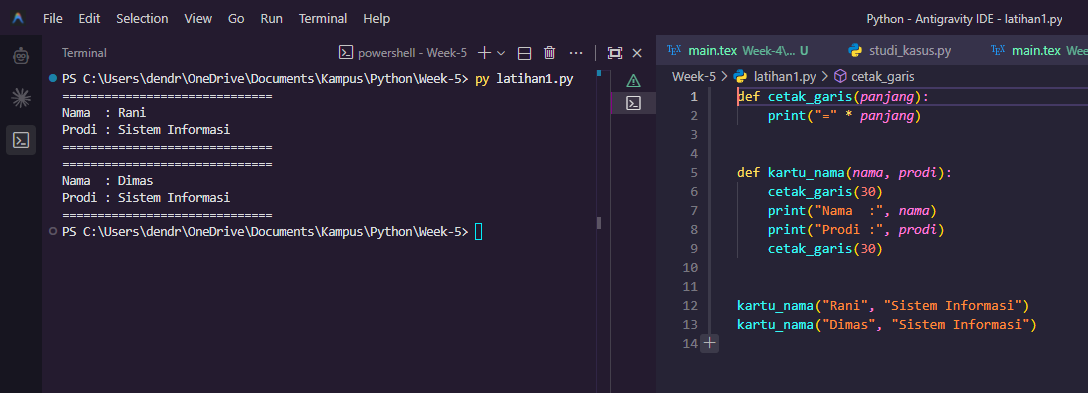
\includegraphics[width=0.85\textwidth]{image/latihan1.png}%
    }{%
        \imageplaceholder{Output Percobaan 1: Prosedur dan Komposisi Fungsi}%
    }
    \caption{Hasil/Output Percobaan 1: Prosedur dan Komposisi Fungsi}
\end{figure}

\subsubsection{Analisis}
Percobaan 1 mendemonstrasikan implementasi prosedur (\textit{void function}) dan konsep komposisi fungsi (*function composition*). Prosedur \texttt{cetak\_garis} dan \texttt{kartu\_nama} tidak memiliki klausa \texttt{return}. Jika nilai hasil pemanggilan fungsi tersebut ditampung ke dalam variabel (misalnya $x = \text{kartu\_nama(...)}$), variabel $x$ akan berisi objek bawaan \texttt{None}.

Meskipun tidak mengembalikan nilai data, prosedur ini memberikan modularitas tinggi melalui pemanfaatan parameter formal. Prosedur \texttt{kartu\_nama} menggunakan parameter dinamis (\texttt{nama} dan \texttt{prodi}) untuk merender identitas yang berbeda dengan format tata letak yang identik, sekaligus memanggil prosedur lain (\texttt{cetak\_garis(30)}) di dalamnya. Operator replikasi string \texttt{"=" * panjang} menyederhanakan pembuatan garis pemisah tanpa memerlukan perulangan eksplisit. Hal ini secara efektif mencegah duplikasi penulisan kode (*boilerplate*) pada program.

\subsection{Percobaan 2: Fungsi dengan Nilai Kembalian dan Komputasi Numerik}
\subsubsection{Algoritma}
\begin{enumerate}
    \item Mulai program.
    \item Definisikan fungsi \texttt{celsius\_ke\_fahrenheit(c)} yang mengembalikan nilai numerik formula $c \times 9 / 5 + 32$.
    \item Definisikan fungsi \texttt{luas\_persegi\_panjang(p, l)} yang mengembalikan hasil perkalian skalar $p \times l$.
    \item Minta masukan nilai float suhu Celsius dari konsol dan simpan ke variabel \texttt{suhu}.
    \item Panggil fungsi \texttt{celsius\_ke\_fahrenheit(suhu)}, simpan nilainya ke variabel \texttt{f}, dan cetak hasilnya.
    \item Panggil fungsi \texttt{luas\_persegi\_panjang(4, 3)} dan simpan ke variabel \texttt{luas\_kamar}.
    \item Panggil fungsi \texttt{luas\_persegi\_panjang(3, 2)} dan simpan ke variabel \texttt{luas\_dapur}.
    \item Tampilkan nilai masing-masing luas ruangan serta cetak hasil penjumlahan ekspresi $luas\_kamar + luas\_dapur$.
    \item Selesai.
\end{enumerate}

\subsubsection{Hasil / Output}
\begin{figure}[H]
    \centering
    \IfFileExists{image/latihan2.png}{%
        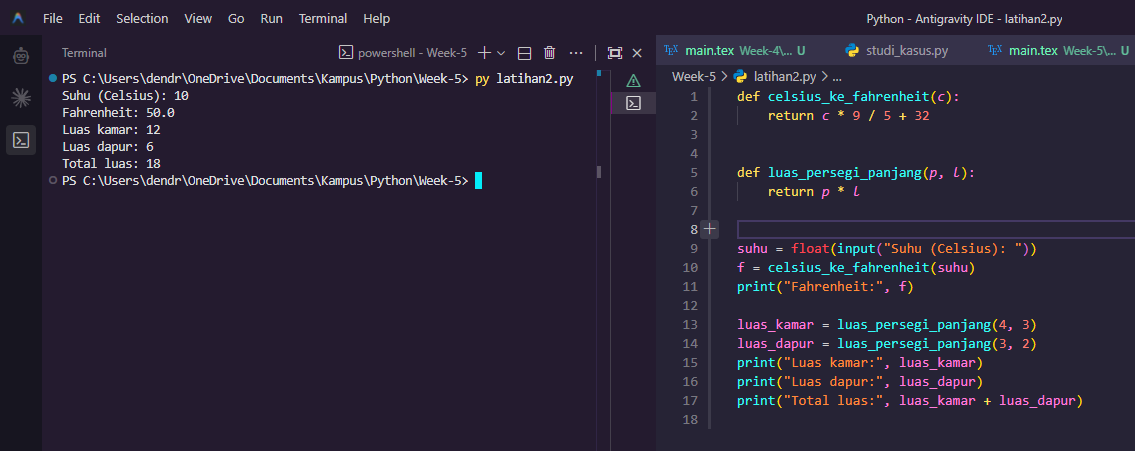
\includegraphics[width=0.85\textwidth]{image/latihan2.png}%
    }{%
        \imageplaceholder{Output Percobaan 2: Nilai Kembalian dan Komputasi Numerik}%
    }
    \caption{Hasil/Output Percobaan 2: Nilai Kembalian dan Komputasi Numerik}
\end{figure}

\subsubsection{Analisis}
Percobaan 2 menggarisbawahi kegunaan utama instruksi \texttt{return}. Berbeda dengan fungsi yang hanya melakukan pencetakan via \texttt{print()}, fungsi bernilai kembali mentransformasikan fungsi menjadi produsen data yang dapat berpartisipasi dalam ekspresi matematika lanjutan.

Sebagai contoh, fungsi \texttt{luas\_persegi\_panjang(p, l)} dipanggil dua kali dengan pasangan argumen yang berbeda: $(4, 3)$ menghasilkan nilai integer 12 untuk \texttt{luas\_kamar}, dan $(3, 2)$ menghasilkan nilai 6 untuk \texttt{luas\_dapur}. Karena kedua nilai tersebut berhasil ditampung dalam variabel pemanggil, program dapat secara langsung mengeksekusi operasi penjumlahan aritmatika tingkat lanjut \texttt{luas\_kamar + luas\_dapur} yang menghasilkan total luas 18. Mekanisme ini memisahkan logika komputasi data dari logika presentasi antarmuka.

\subsection{Percobaan 3: Percabangan Bersyarat dalam Fungsi dan Predikat Boolean}
\subsubsection{Algoritma}
\begin{enumerate}
    \item Mulai program.
    \item Definisikan fungsi konversi grade \texttt{nilai\_huruf(nilai)} dengan rantai \texttt{if-elif} berpemutusan dini (*early return*).
    \item Definisikan fungsi predikat \texttt{lulus(nilai)} yang mengembalikan hasil evaluasi boolean dari relasi komparasi $nilai \ge 55$.
    \item Lakukan perulangan \texttt{for} sebanyak 3 kali iterasi:
    \begin{enumerate}[label=\alph*.]
        \item Baca masukan bilangan integer \texttt{n}.
        \item Uji kondisi dengan memanggil fungsi predikat: \texttt{if lulus(n):} tetapkan $status = \text{"Lulus"}$, selain itu tetapkan $status = \text{"Tidak lulus"}$.
        \item Cetak nilai \texttt{n}, tanda panah, hasil pemanggilan fungsi \texttt{nilai\_huruf(n)}, serta teks \texttt{status}.
    \end{enumerate}
    \item Selesai.
\end{enumerate}

\subsubsection{Hasil / Output}
\begin{figure}[H]
    \centering
    \IfFileExists{image/latihan3.png}{%
        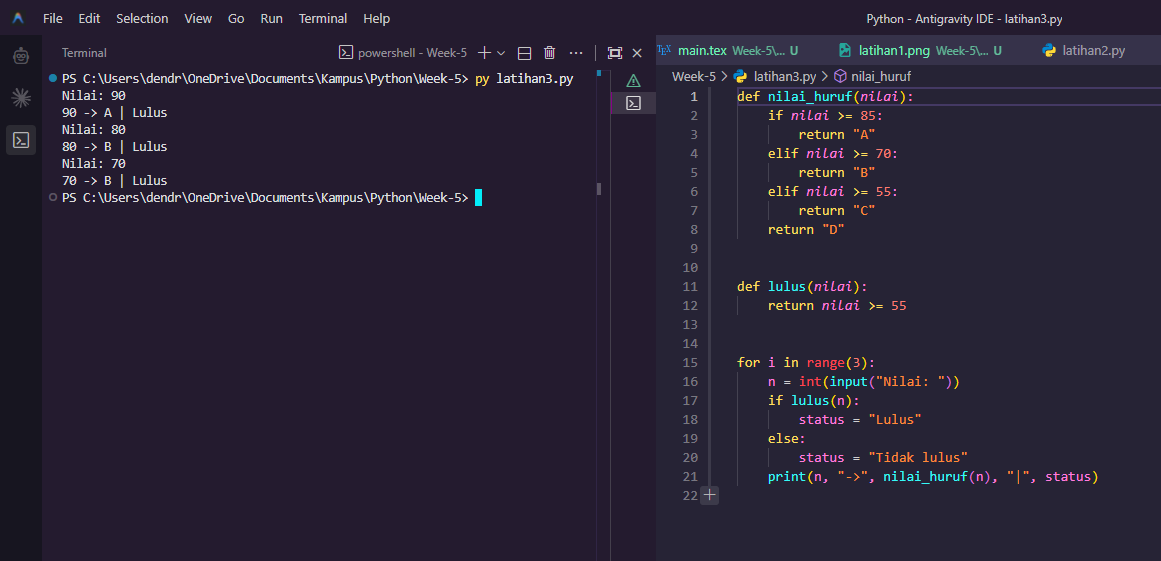
\includegraphics[width=0.85\textwidth]{image/latihan3.png}%
    }{%
        \imageplaceholder{Output Percobaan 3: Predikat Boolean dan Early Return}%
    }
    \caption{Hasil/Output Percobaan 3: Predikat Boolean dan Early Return}
\end{figure}

\subsubsection{Analisis}
Percobaan 3 mengimplementasikan dua pola arsitektur fungsi yang sangat efisien:
\begin{enumerate}
    \item \textbf{Pola Pemutusan Dini (\textit{Early Return Pattern})}: Pada fungsi \texttt{nilai\_huruf}, begitu suatu kondisi terpenuhi (misalnya $nilai \ge 85$), kata kunci \texttt{return "A"} seketika menghentikan eksekusi tubuh fungsi dan mengembalikan nilai \texttt{"A"}. Tidak diperlukan variabel perantara (\textit{intermediate variable}) atau klausa \texttt{else} penutup yang bersarang terlalu dalam, menghasilkan kode yang bersih dan terhindar dari *anti-pattern arrowhead style*.
    \item \textbf{Fungsi Predikat Boolean}: Fungsi \texttt{lulus(nilai)} mengembalikan objek boolean murni (\texttt{True} atau \texttt{False}) dari ekspresi relasional $nilai \ge 55$. Penggunaan fungsi predikat ini menyederhanakan klausa kondisional pada program utama menjadi \texttt{if lulus(n):}, yang sangat ekspresif dan menyerupai bahasa alami (*self-documenting code*).
\end{enumerate}

\subsection{Percobaan 4: Integrasi Pustaka Standar math dan random}
\subsubsection{Algoritma}
\begin{enumerate}
    \item Mulai program.
    \item Impor pustaka bawaan sistem: modul \texttt{math} dan modul \texttt{random}.
    \item Rancang fungsi kustom \texttt{jarak(x1, y1, x2, y2)} yang memformulasikan jarak Euclidean melalui pemanggilan fungsi \texttt{math.sqrt((x2 - x1)**2 + (y2 - y1)**2)}.
    \item Rancang fungsi kustom \texttt{lempar\_dadu()} yang memanggil fungsi generator bilangan acak semu \texttt{random.randint(1, 6)}.
    \item Evaluasi dan cetak jarak titik $(0,0)$ ke $(3,4)$.
    \item Evaluasi jarak titik $(1,1)$ ke $(4, 5.5)$, lakukan pembulatan ke bilangan bulat terdekat di atasnya via fungsi \texttt{math.ceil()}, dan cetak hasilnya.
    \item Lakukan iterasi perulangan sebanyak 3 kali untuk mencetak hasil pengacakan dadu via fungsi \texttt{lempar\_dadu()}.
    \item Selesai.
\end{enumerate}

\subsubsection{Hasil / Output}
\begin{figure}[H]
    \centering
    \IfFileExists{image/latihan4.png}{%
        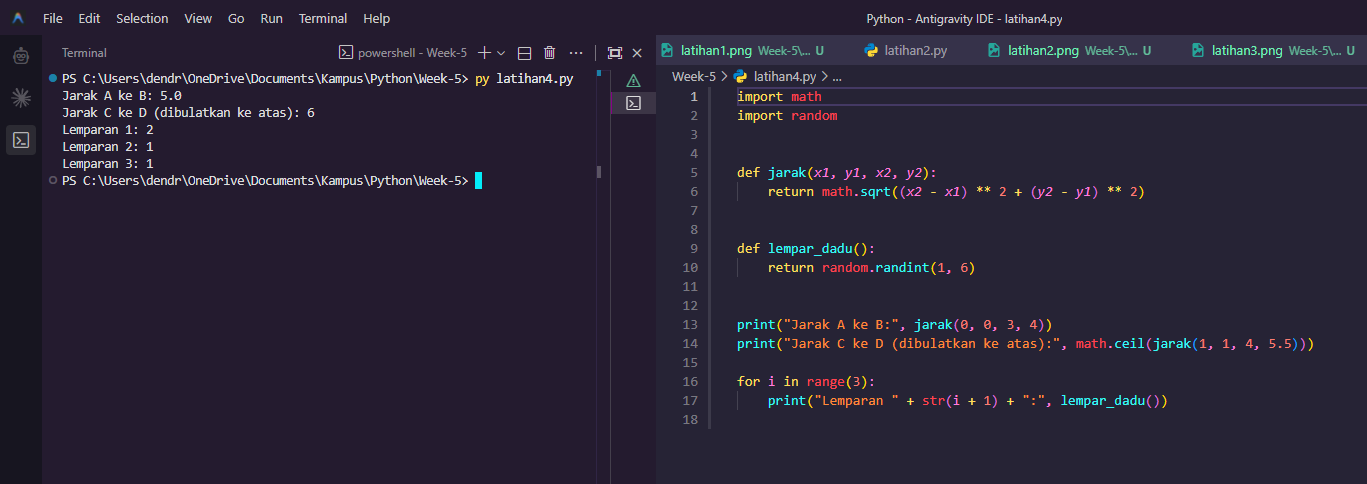
\includegraphics[width=0.85\textwidth]{image/latihan4.png}%
    }{%
        \imageplaceholder{Output Percobaan 4: Pustaka Standar math dan random}%
    }
    \caption{Hasil/Output Percobaan 4: Pustaka Standar math dan random}
\end{figure}

\subsubsection{Analisis}
Percobaan 4 membuktikan keandalan ekosistem modul bawaan (*standard library*) pada Python 3. Pembuatan fungsi kustom yang membungkus fungsi pustaka standar (*wrapper function*) memberikan abstraksi tingkat tinggi:
\begin{itemize}
    \item Pada kalkulasi jarak Euclidean titik $(0,0)$ ke $(3,4)$, formula matematika $\sqrt{(3-0)^2 + (4-0)^2} = \sqrt{9+16} = \sqrt{25} = 5.0$ dihitung secara deterministik dan berpresisi tinggi oleh \texttt{math.sqrt}.
    \item Pada penghitungan jarak titik $(1,1)$ ke $(4, 5.5)$, nilai riil yang dihasilkan adalah $\sqrt{3^2 + 4.5^2} = \sqrt{9 + 20.25} = \sqrt{29.25} \approx 5.4083$. Penerapan fungsi plafon \texttt{math.ceil()} membulatkan nilai tersebut ke atas menuju bilangan bulat terdekat yaitu $6$.
    \item Fungsi \texttt{random.randint(1, 6)} memanfaatkan algoritma *Mersenne Twister* bawaan Python untuk membangkitkan bilangan bulat acak yang terdistribusi secara seragam pada interval tertutup $[1, 6]$. Hal ini mendemonstrasikan integrasi komputasi deterministik dan stokastik dalam pemrograman terstruktur.
\end{itemize}

\subsection{Percobaan 5: Fungsi Rekursif dan Penentuan Base Case}
\subsubsection{Algoritma}
\begin{enumerate}
    \item Mulai program.
    \item Definisikan fungsi rekursif \texttt{faktorial(n)}:
    \begin{enumerate}[label=\alph*.]
        \item Kasus Basis: jika $n == 0$, kembalikan nilai 1.
        \item Kasus Rekursif: selain itu, kembalikan ekspresi $n \times \text{faktorial}(n - 1)$.
    \end{enumerate}
    \item Definisikan prosedur rekursif \texttt{hitung\_mundur(n)}:
    \begin{enumerate}[label=\alph*.]
        \item Kasus Basis: jika $n == 0$, cetak string \texttt{"Mulai!"}.
        \item Kasus Rekursif: selain itu, cetak nilai $n$ dan panggil \texttt{hitung\_mundur(n - 1)}.
    \end{enumerate}
    \item Evaluasi dan cetak hasil perhitungan faktorial dari bilangan 5: \texttt{faktorial(5)}.
    \item Eksekusi prosedur hitung mundur mulai dari angka 3: \texttt{hitung\_mundur(3)}.
    \item Selesai.
\end{enumerate}

\subsubsection{Hasil / Output}
\begin{figure}[H]
    \centering
    \IfFileExists{image/latihan5.png}{%
        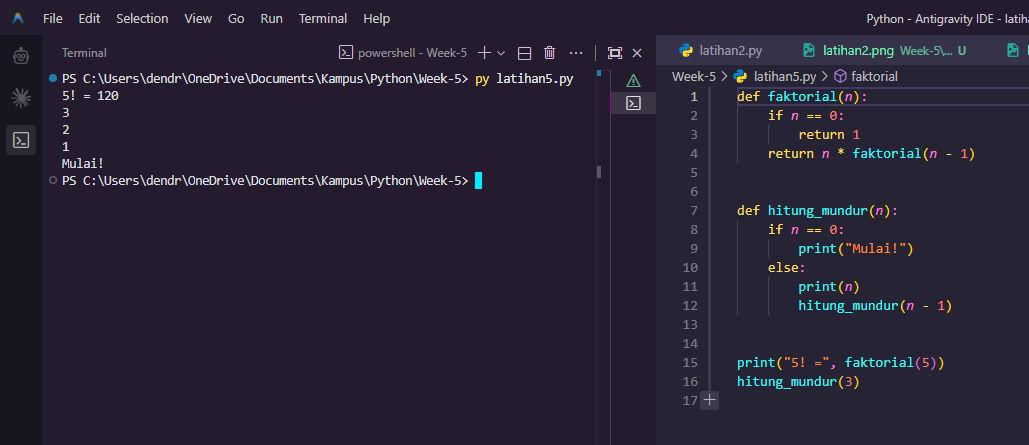
\includegraphics[width=0.85\textwidth]{image/latihan5.png}%
    }{%
        \imageplaceholder{Output Percobaan 5: Fungsi Rekursif dan Base Case}%
    }
    \caption{Hasil/Output Percobaan 5: Fungsi Rekursif dan Base Case}
\end{figure}

\subsubsection{Analisis}
Percobaan 5 mendalami konsep rekursi (*recursion*). Eksekusi fungsi rekursif mengandalkan struktur data tumpukan pemanggilan (*call stack*). Pada pemanggilan \texttt{faktorial(5)}, Python menumpuk bingkai fungsi secara bertingkat:
\begin{equation}
5 \times \text{faktorial}(4) \to 4 \times \text{faktorial}(3) \to 3 \times \text{faktorial}(2) \to 2 \times \text{faktorial}(1) \to 1 \times \text{faktorial}(0)
\end{equation}
Saat $n = 0$, kondisi kasus basis (*base case*) $n == 0$ terpenuhi sehingga fungsi mengembalikan nilai skalar 1 tanpa melakukan pemanggilan rekursif lanjutan. Selanjutnya, fase pelepasan tumpukan (*stack unwinding*) berlangsung di mana nilai-nilai parsial dikalikan mundur: $1 \times 1 = 1 \to 2 \times 1 = 2 \to 3 \times 2 = 6 \to 4 \times 6 = 24 \to 5 \times 24 = 120$.

Keberadaan kasus basis merupakan prasyarat mutlak dalam algoritma rekursif. Apabila kasus basis diabaikan atau kondisi tidak pernah tercapai, perulangan pemanggilan akan terus bertambah hingga melampaui batas kedalaman tumpukan memori interpreter Python (secara bawaan 1000 lapis), yang memicu galat kritis \texttt{RecursionError: maximum recursion depth exceeded}.

\subsection{Percobaan 6: Studi Kasus Kalkulator Nilai Akhir Mahasiswa}
\subsubsection{Algoritma}
\begin{enumerate}
    \item Mulai program.
    \item Rancang lima modul fungsi independen:
    \begin{enumerate}[label=\alph*.]
        \item \texttt{nilai\_valid(n)}: memeriksa rentang $0 \le n \le 100$.
        \item \texttt{baca\_nilai(label)}: membaca masukan berulang selama data tidak valid.
        \item \texttt{nilai\_akhir(tugas, uts, uas)}: menghitung kombinasi linear berbobot 30\% Tugas, 30\% UTS, dan 40\% UAS.
        \item \texttt{nilai\_huruf(na)}: mengklasifikasikan nilai angka ke grade A, B, C, atau D.
        \item \texttt{rata\_rata(total, banyak)}: menghitung pembagian aman dengan pengembalian 0 saat $banyak == 0$.
    \end{enumerate}
    \item Masuk ke blok utama: baca jumlah mahasiswa, inisialisasi $jumlah\_lulus = 0$ dan $total\_nilai = 0$.
    \item Jalankan perulangan \texttt{for} untuk setiap mahasiswa: baca nama, baca komponen nilai terbobot via \texttt{baca\_nilai()}, kalkulasikan $na$, tentukan $huruf$, tambahkan ke akumulator, dan cetak rincian individu.
    \item Tampilkan kuantitas kelulusan dan nilai rata-rata akhir kelas.
    \item Selesai.
\end{enumerate}

\subsubsection{Hasil / Output}
\begin{figure}[H]
    \centering
    \IfFileExists{image/studi_kasus.png}{%
        \includegraphics[width=0.85\textwidth]{image/studi_kasus.png}%
    }{%
        \IfFileExists{image/latihan6.png}{%
            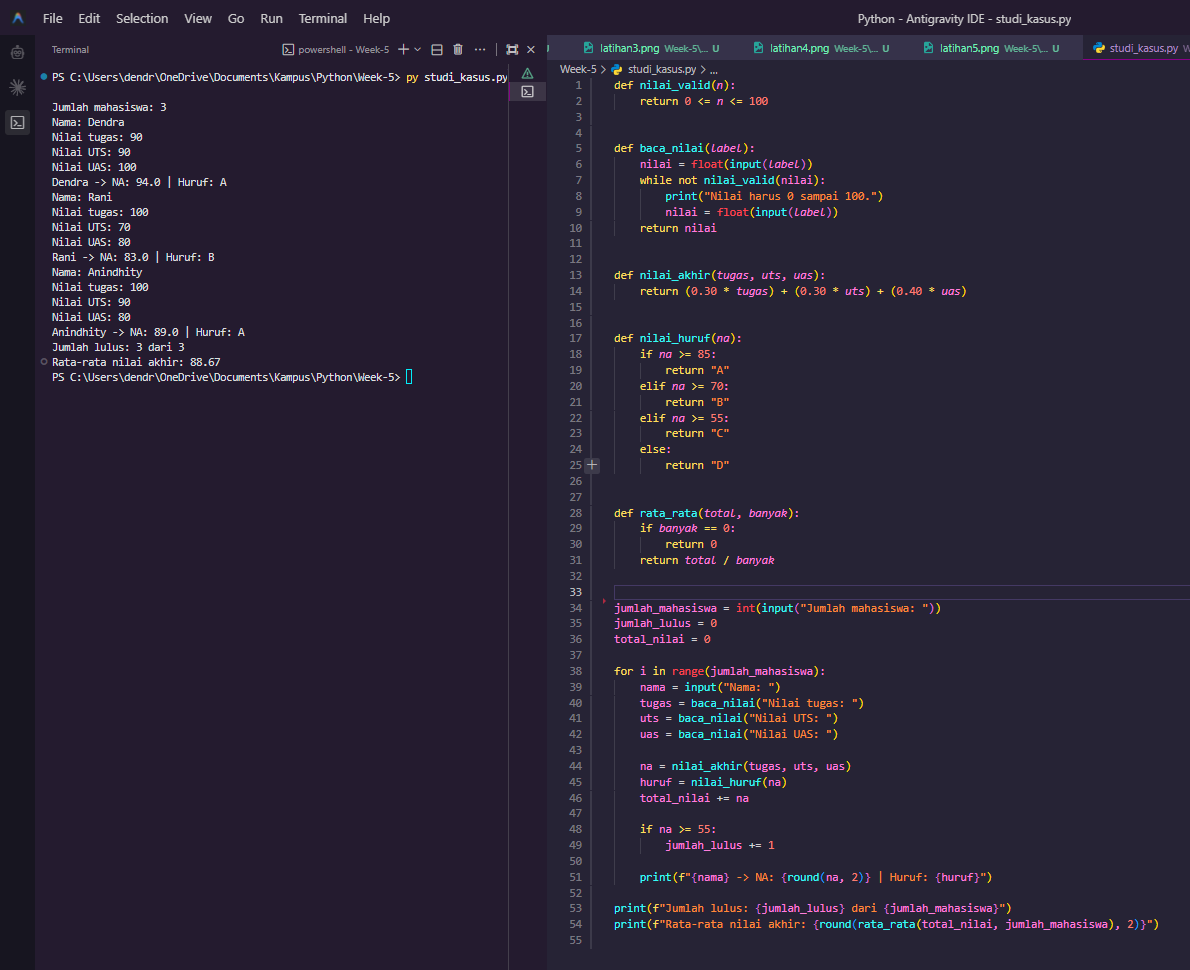
\includegraphics[width=0.85\textwidth]{image/latihan6.png}%
        }{%
            \imageplaceholder{Output Percobaan 6: Studi Kasus Kalkulator Nilai Akhir}%
        }%
    }
    \caption{Hasil/Output Percobaan 6: Studi Kasus Kalkulator Nilai Akhir}
\end{figure}

\subsubsection{Analisis}
Studi kasus ini merepresentasikan implementasi nyata dari arsitektur perangkat lunak berbasis fungsi (*modular function decomposition*). Program dipecah menjadi tanggung jawab tunggal (*Single Responsibility Principle*):
\begin{enumerate}
    \item \textbf{Validasi Masukan Terisolasi}: Fungsi \texttt{baca\_nilai} memanfaatkan komposisi fungsi predikat \texttt{nilai\_valid}. Logika validasi rentang tertutup $[0, 100]$ hanya didefinisikan satu kali, namun digunakan berulang untuk membaca nilai Tugas, UTS, dan UAS. Hal ini mengeliminasi duplikasi kode secara drastis.
    \item \textbf{Kalkulasi Nilai Terbobot Deterministik}: Pemisahan formula matematika pada fungsi \texttt{nilai\_akhir} memudahkan perubahan kebijakan bobot di masa depan tanpa perlu memodifikasi alur pembacaan data masukan atau logika penyajian luaran.
    \item \textbf{Ketahanan Komputasi Terhadap Zero Division}: Pemanfaatan fungsi \texttt{rata\_rata} yang membungkus pengujian kondisi $banyak == 0$ menjamin program tidak akan mengalami kegagalan sistem (*crash*) apabila pengguna menginputkan jumlah mahasiswa sebanyak 0 orang.
\end{enumerate}
Dengan demikian, program utama menjadi sangat ringkas, terstruktur, dan memiliki tingkat keterbacaan serta kemudahan pemeliharaan (*maintainability*) yang optimal.

% ============================================================
% KESIMPULAN
% ============================================================
\section{KESIMPULAN}
Berdasarkan serangkaian percobaan, eksplorasi teoritis, dan studi kasus yang dilakukan pada Praktikum Modul 5, dapat ditarik beberapa kesimpulan penting sebagai berikut:
\begin{enumerate}
    \item Pemrograman modular menggunakan fungsi (\texttt{def}) meningkatkan keterbacaan, keandalan, dan kemudahan pemeliharaan kode perangkat lunak melalui penerapan prinsip \textit{reusability} dan eliminasi redundansi kode (prinsip DRY).
    \item Prosedur (\textit{void function}) bertindak sebagai pengelola alur aksi dan presentasi keluaran konsol yang secara implisit mengembalikan nilai \texttt{None}, sedangkan fungsi bernilai kembali (\texttt{return}) bertindak sebagai produsen data yang mentransmisikan nilai komputasi untuk diproses lebih lanjut.
    \item Penerapan pola pemutusan dini (*early return*) pada percabangan bersyarat membuat struktur logika lebih linier dan menghilangkan kebutuhan terhadap blok percabangan bersarang yang kompleks (*nested blocks*).
    \item Pustaka standar Python seperti modul \texttt{math} dan \texttt{random} menyediakan fungsi matematis dan stokastik bawaan yang telah teroptimasi, sehingga dapat langsung diintegrasikan ke dalam fungsi kustom dengan presisi komputasi tinggi.
    \item Algoritma rekursif menuntut identifikasi kasus basis (*base case*) yang ketat dan deterministik untuk memastikan proses pemanggilan diri sendiri berhenti secara aman sebelum melampaui batas kedalaman tumpukan memori (*stack overflow*).
    \item Komposisi fungsi pembantu yang berpegang pada prinsip tanggung jawab tunggal (*Single Responsibility Principle*), seperti fungsi validasi masukan dan pelindung pembagian dengan nol, menghasilkan arsitektur program yang kokoh (*robust*) dan mudah diperluas (*scalable*).
\end{enumerate}

% ============================================================
% DAFTAR PUSTAKA
% ============================================================
\section{DAFTAR PUSTAKA}

\begin{enumerate}
    \item Tim Dosen Algoritma dan Pemrograman. (2025). \textit{Modul Praktikum 5: Fungsi, Parameter, dan Nilai Kembalian}. Program Studi S1 Sistem Informasi, Fakultas Rekayasa Industri, Telkom University Surabaya.

    \item Python Software Foundation. (2024). \textit{Defining Functions - Python 3.12 Documentation}. Diakses dari \url{https://docs.python.org/3/tutorial/controlflow.html#defining-functions}.

    \item Lutz, M. (2013). \textit{Learning Python (5th Edition)}. O'Reilly Media.

    \item Martin, R. C. (2008). \textit{Clean Code: A Handbook of Agile Software Craftsmanship}. Prentice Hall.
\end{enumerate}

\end{document}
